\documentclass[tikz,border=2pt]{standalone}
\usepackage{amsmath,amssymb}
\usepackage{pgfplots}
\pgfplotsset{compat=1.18}
\usetikzlibrary{arrows.meta}

\begin{document}
% q(h) = h_1^2 - h_2^2 is indefinite on R^2 (hyperbolas, both signs), yet restricted to the
% constraint directions T = {h : h_1 - 2h_2 = 0} it is positive: along that line q = 3 h_2^2.
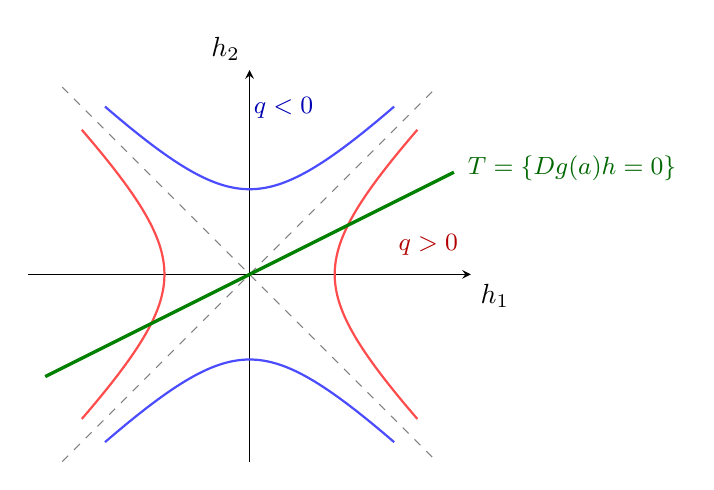
\begin{tikzpicture}
	\begin{axis}[
		axis lines=middle, axis equal image, xmin=-2.6, xmax=2.6, ymin=-2.2, ymax=2.4,
		xtick=\empty, ytick=\empty, xlabel={$h_1$}, ylabel={$h_2$}, xlabel style={below right}, ylabel style={above left},
		samples=80, clip=false, width=7.6cm
		]
		\addplot[red!70, thick, domain=-1.3:1.3] ({cosh(x)}, {sinh(x)});
		\addplot[red!70, thick, domain=-1.3:1.3] ({-cosh(x)}, {sinh(x)});
		\addplot[blue!70, thick, domain=-1.3:1.3] ({sinh(x)}, {cosh(x)});
		\addplot[blue!70, thick, domain=-1.3:1.3] ({sinh(x)}, {-cosh(x)});
		\addplot[gray, dashed, domain=-2.2:2.2, samples=2] {x};
		\addplot[gray, dashed, domain=-2.2:2.2, samples=2] {-x};
		\addplot[green!50!black, very thick, domain=-2.4:2.4, samples=2] {x/2};
		\node[red!70!black, font=\small] at (axis cs:2.1,0.35) {$q>0$};
		\node[blue!70!black, font=\small] at (axis cs:0.4,1.95) {$q<0$};
		\node[green!40!black, font=\small, anchor=west] at (axis cs:2.45,1.25) {$T=\{Dg(a)h=0\}$};
	\end{axis}
\end{tikzpicture}
\end{document}
